% GNUPLOT: LaTeX picture with Postscript
\begingroup
  \makeatletter
  \providecommand\color[2][]{%
    \GenericError{(gnuplot) \space\space\space\@spaces}{%
      Package color not loaded in conjunction with
      terminal option `colourtext'%
    }{See the gnuplot documentation for explanation.%
    }{Either use 'blacktext' in gnuplot or load the package
      color.sty in LaTeX.}%
    \renewcommand\color[2][]{}%
  }%
  \providecommand\includegraphics[2][]{%
    \GenericError{(gnuplot) \space\space\space\@spaces}{%
      Package graphicx or graphics not loaded%
    }{See the gnuplot documentation for explanation.%
    }{The gnuplot epslatex terminal needs graphicx.sty or graphics.sty.}%
    \renewcommand\includegraphics[2][]{}%
  }%
  \providecommand\rotatebox[2]{#2}%
  \@ifundefined{ifGPcolor}{%
    \newif\ifGPcolor
    \GPcolorfalse
  }{}%
  \@ifundefined{ifGPblacktext}{%
    \newif\ifGPblacktext
    \GPblacktexttrue
  }{}%
  % define a \g@addto@macro without @ in the name:
  \let\gplgaddtomacro\g@addto@macro
  % define empty templates for all commands taking text:
  \gdef\gplbacktext{}%
  \gdef\gplfronttext{}%
  \makeatother
  \ifGPblacktext
    % no textcolor at all
    \def\colorrgb#1{}%
    \def\colorgray#1{}%
  \else
    % gray or color?
    \ifGPcolor
      \def\colorrgb#1{\color[rgb]{#1}}%
      \def\colorgray#1{\color[gray]{#1}}%
      \expandafter\def\csname LTw\endcsname{\color{white}}%
      \expandafter\def\csname LTb\endcsname{\color{black}}%
      \expandafter\def\csname LTa\endcsname{\color{black}}%
      \expandafter\def\csname LT0\endcsname{\color[rgb]{1,0,0}}%
      \expandafter\def\csname LT1\endcsname{\color[rgb]{0,1,0}}%
      \expandafter\def\csname LT2\endcsname{\color[rgb]{0,0,1}}%
      \expandafter\def\csname LT3\endcsname{\color[rgb]{1,0,1}}%
      \expandafter\def\csname LT4\endcsname{\color[rgb]{0,1,1}}%
      \expandafter\def\csname LT5\endcsname{\color[rgb]{1,1,0}}%
      \expandafter\def\csname LT6\endcsname{\color[rgb]{0,0,0}}%
      \expandafter\def\csname LT7\endcsname{\color[rgb]{1,0.3,0}}%
      \expandafter\def\csname LT8\endcsname{\color[rgb]{0.5,0.5,0.5}}%
    \else
      % gray
      \def\colorrgb#1{\color{black}}%
      \def\colorgray#1{\color[gray]{#1}}%
      \expandafter\def\csname LTw\endcsname{\color{white}}%
      \expandafter\def\csname LTb\endcsname{\color{black}}%
      \expandafter\def\csname LTa\endcsname{\color{black}}%
      \expandafter\def\csname LT0\endcsname{\color{black}}%
      \expandafter\def\csname LT1\endcsname{\color{black}}%
      \expandafter\def\csname LT2\endcsname{\color{black}}%
      \expandafter\def\csname LT3\endcsname{\color{black}}%
      \expandafter\def\csname LT4\endcsname{\color{black}}%
      \expandafter\def\csname LT5\endcsname{\color{black}}%
      \expandafter\def\csname LT6\endcsname{\color{black}}%
      \expandafter\def\csname LT7\endcsname{\color{black}}%
      \expandafter\def\csname LT8\endcsname{\color{black}}%
    \fi
  \fi
  \setlength{\unitlength}{0.0500bp}%
  \begin{picture}(7200.00,4364.00)%
    \gplgaddtomacro\gplbacktext{%
      \csname LTb\endcsname%
      \put(1386,704){\makebox(0,0)[r]{\strut{}$"0"$}}%
      \put(1386,1204){\makebox(0,0)[r]{\strut{}$"100"$}}%
      \put(1386,1704){\makebox(0,0)[r]{\strut{}$"200"$}}%
      \put(1386,2204){\makebox(0,0)[r]{\strut{}$"300"$}}%
      \put(1386,2704){\makebox(0,0)[r]{\strut{}$"400"$}}%
      \put(1386,3204){\makebox(0,0)[r]{\strut{}$"500"$}}%
      \put(1386,3704){\makebox(0,0)[r]{\strut{}$"600"$}}%
      \put(1518,484){\makebox(0,0){\strut{}$"0"$}}%
      \put(2359,484){\makebox(0,0){\strut{}$"12"$}}%
      \put(3200,484){\makebox(0,0){\strut{}$"24"$}}%
      \put(748,2204){\rotatebox{90}{\makebox(0,0){\strut{}\popi{V}{\%}}}}%
      \put(2394,154){\makebox(0,0){\strut{}\popi{t}{hod}}}%
      \put(2394,4034){\makebox(0,0){\strut{}Jojo}}%
    }%
    \gplgaddtomacro\gplfronttext{%
      \csname LTb\endcsname%
      \put(2283,1757){\makebox(0,0)[r]{\strut{}norm�ln�}}%
      \csname LTb\endcsname%
      \put(2283,1537){\makebox(0,0)[r]{\strut{}slan�}}%
      \csname LTb\endcsname%
      \put(2283,1317){\makebox(0,0)[r]{\strut{}sladk�}}%
      \csname LTb\endcsname%
      \put(2283,1097){\makebox(0,0)[r]{\strut{}studen�}}%
      \csname LTb\endcsname%
      \put(2283,877){\makebox(0,0)[r]{\strut{}nasycen� r.}}%
    }%
    \gplgaddtomacro\gplbacktext{%
      \csname LTb\endcsname%
      \put(4986,704){\makebox(0,0)[r]{\strut{}$"0"$}}%
      \put(4986,1204){\makebox(0,0)[r]{\strut{}$"100"$}}%
      \put(4986,1704){\makebox(0,0)[r]{\strut{}$"200"$}}%
      \put(4986,2204){\makebox(0,0)[r]{\strut{}$"300"$}}%
      \put(4986,2704){\makebox(0,0)[r]{\strut{}$"400"$}}%
      \put(4986,3204){\makebox(0,0)[r]{\strut{}$"500"$}}%
      \put(4986,3704){\makebox(0,0)[r]{\strut{}$"600"$}}%
      \put(5118,484){\makebox(0,0){\strut{}$"0"$}}%
      \put(5959,484){\makebox(0,0){\strut{}$"12"$}}%
      \put(6800,484){\makebox(0,0){\strut{}$"24"$}}%
      \put(4348,2204){\rotatebox{90}{\makebox(0,0){\strut{}\popi{V}{\%}}}}%
      \put(5994,154){\makebox(0,0){\strut{}\popi{t}{hod}}}%
      \put(5994,4034){\makebox(0,0){\strut{}Haribo}}%
    }%
    \gplgaddtomacro\gplfronttext{%
      \csname LTb\endcsname%
      \put(5883,1757){\makebox(0,0)[r]{\strut{}norm�ln�}}%
      \csname LTb\endcsname%
      \put(5883,1537){\makebox(0,0)[r]{\strut{}slan�}}%
      \csname LTb\endcsname%
      \put(5883,1317){\makebox(0,0)[r]{\strut{}sladk�}}%
      \csname LTb\endcsname%
      \put(5883,1097){\makebox(0,0)[r]{\strut{}studen�}}%
      \csname LTb\endcsname%
      \put(5883,877){\makebox(0,0)[r]{\strut{}nasycen� r.}}%
    }%
    \gplbacktext
    \put(0,0){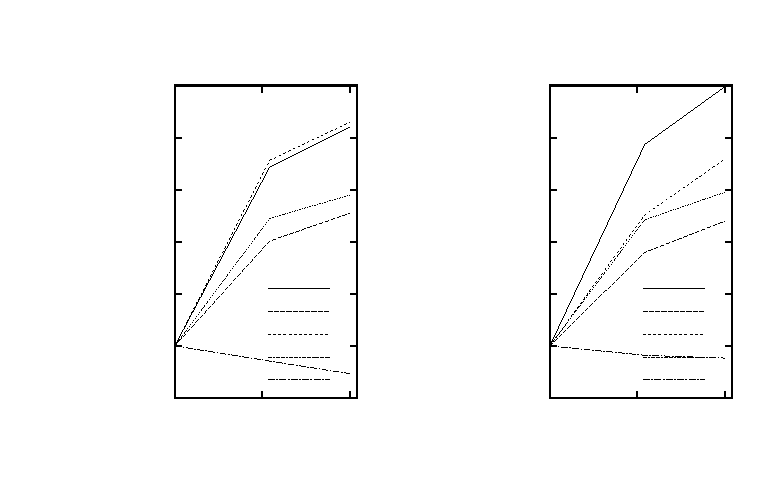
\includegraphics{problem1-7-data}}%
    \gplfronttext
  \end{picture}%
\endgroup
